%% LyX 2.3.6.1 created this file.  For more info, see http://www.lyx.org/.
%% Do not edit unless you really know what you are doing.
\documentclass[10pt,english,t,10pt]{beamer}
\usepackage{lmodern}
\usepackage[T1]{fontenc}
\usepackage[utf8]{inputenc}
\setcounter{tocdepth}{1}
\setlength{\parskip}{\smallskipamount}
\setlength{\parindent}{0pt}
\usepackage{amsbsy}
\usepackage{amstext}
\usepackage{amssymb}
\usepackage{graphicx}
\usepackage[authoryear]{natbib}

\makeatletter
%%%%%%%%%%%%%%%%%%%%%%%%%%%%%% Textclass specific LaTeX commands.
% this default might be overridden by plain title style
\newcommand\makebeamertitle{\frame{\maketitle}}%
% (ERT) argument for the TOC
\AtBeginDocument{%
  \let\origtableofcontents=\tableofcontents
  \def\tableofcontents{\@ifnextchar[{\origtableofcontents}{\gobbletableofcontents}}
  \def\gobbletableofcontents#1{\origtableofcontents}
}

%%%%%%%%%%%%%%%%%%%%%%%%%%%%%% User specified LaTeX commands.



\usepackage{tikz}
\usetikzlibrary{positioning}
\usepackage{appendixnumberbeamer}

\usepackage{graphicx}
\usepackage{subfig}

\usetheme[progressbar=frametitle,block=fill,subsectionpage=progressbar]{metropolis}

% margin
\setbeamersize{text margin right=1.5cm}

% colors
\definecolor{DarkRed}{rgb}{0.7,0,0}
%\colorlet{DarkRed}{red!70!black}
\setbeamercolor{normal text}{fg=black}
\setbeamercolor{alerted text}{fg=DarkRed}
\setbeamercolor{progress bar}{fg=DarkRed}
\setbeamercolor{button}{bg=DarkRed}

% width of seperators
\makeatletter
\setlength{\metropolis@titleseparator@linewidth}{1pt}
\setlength{\metropolis@progressonsectionpage@linewidth}{1pt}
\setlength{\metropolis@progressinheadfoot@linewidth}{1pt}
\makeatother

% new alert block
\newlength\origleftmargini
\setlength\origleftmargini\leftmargini
\setbeamertemplate{itemize/enumerate body begin}{\setlength{\leftmargini}{4mm}}
\let\oldalertblock\alertblock
\let\oldendalertblock\endalertblock
\def\alertblock{\begingroup \setbeamertemplate{itemize/enumerate body begin}{\setlength{\leftmargini}{\origleftmargini}} \oldalertblock}
\def\endalertblock{\oldendalertblock \endgroup}
\setbeamertemplate{mini frame}{}
\setbeamertemplate{mini frame in current section}{}
\setbeamertemplate{mini frame in current subsection}{}
\setbeamercolor{section in head/foot}{fg=normal text.bg, bg=structure.fg}
\setbeamercolor{subsection in head/foot}{fg=normal text.bg, bg=structure.fg}

% footer
\makeatletter
\setbeamertemplate{footline}{%
    \begin{beamercolorbox}[colsep=1.5pt]{upper separation line head}
    \end{beamercolorbox}
    \begin{beamercolorbox}{section in head/foot}
      \vskip1pt\insertsectionnavigationhorizontal{\paperwidth}{}{\hskip0pt plus1filll \insertframenumber{} / \inserttotalframenumber \hskip2pt}\vskip3pt% 
    \end{beamercolorbox}%
    \begin{beamercolorbox}[colsep=1.5pt]{lower separation line head}
    \end{beamercolorbox}
}
\makeatother

% toc
\setbeamertemplate{section in toc}{\hspace*{1em}\inserttocsectionnumber.~\inserttocsection\par}
\setbeamertemplate{subsection in toc}{\hspace*{2em}\inserttocsectionnumber.\inserttocsubsectionnumber.~\inserttocsubsection\par}

\makeatother

\usepackage{babel}
\begin{document}
\title{9. Fiscal Policy in HANK\vspace{-2mm}}
\subtitle{Adv. Macro: Heterogenous Agent Models} 
\author{Nicolai Waldstrøm}
\date{2024}

{
\setbeamertemplate{footline}{} 
\begin{frame}

\maketitle

\begin{tikzpicture}[overlay, remember picture]
\node[above left=0cm and 0.0cm of current page.south east] 
{
\includegraphics[width=4cm]{figs/KUSAMFtitlelrcorner.pdf}};
\end{tikzpicture}

\begin{tikzpicture}[overlay, remember picture]
\node[below left=0.5cm and .8cm of current page.north east] 
{\includegraphics[width=1.5cm]{figs/KUSAMFlogo.pdf}};
\end{tikzpicture}


\end{frame}
}

\addtocounter{framenumber}{-1}

\section{Introduction}
\begin{frame}{Exam info}
\begin{itemize}
\item Exam form:
\begin{itemize}
\item Portfolio (the 3 assignments)
\item \textbf{36 hours} take home
\end{itemize}
\item Exam office thought it was 48 hours, so some dates were wrong online
\begin{itemize}
\item E.g. info in \emph{Exam schedules} at \emph{https://socialsciences.ku.dk/education/studentservices/exam-schedules
}has been \textbf{wrong}
\end{itemize}
\item The correct dates are:
\begin{itemize}
\item Start: January 4th morning (9AM)
\item End: January 5th evening (9PM)
\end{itemize}
\item Re-examination: Oral exam
\end{itemize}
\end{frame}
%
\begin{frame}{Introduction}
\vspace{-2mm}
\begin{itemize}
\item <+->\textbf{Today: }
\begin{itemize}
\item The canonical HANK model
\begin{itemize}
\item Model with sticky wages 
\end{itemize}
\item \textbf{Application}: Fiscal policy in HANK 
\end{itemize}
\item <+->\textbf{Literature: }Auclert et. al. (2023), \\
>>The Intertemporal Keynesian Cross<<
\begin{itemize}
\item Long paper with many (technical) details
\item We will focus on the main results
\end{itemize}
\end{itemize}
\end{frame}
%

\section{Sticky Wages}
\begin{frame}{Detour}
\begin{itemize}
\item <+->Early HANK papers formulated \emph{Heterogeneous Agent New Keynesian}
Models by:
\begin{itemize}
\item Take standard NK model from last lecture
\item Replace Representative agent HH block with Heterogeneous Agents HH
block 
\item See e.g. McKay, Nakamura, and Steinsson (2016), Hagedorn, Manovskii,
and Mitman (2019)
\end{itemize}
\item <+->Turns out that just doing this has undesirable properties when:
\begin{itemize}
\item Prices are sticky
\item Wages are fully flexible
\end{itemize}
\item <+->Need to make one adjustment to standard NK model before adding
HA
\end{itemize}
\end{frame}
%
\begin{frame}{Sticky wages}
\begin{itemize}
\item <+->Canonical NK model features \textbf{sticky} prices\textbf{, flexible}
wages 
\begin{itemize}
\item Fine for some questions, but can cause issues in HA models (see Auclert,
Bardóczy, and Rognlie (2023))
\end{itemize}
\item <+->\textbf{EX}: Standard HA model where households have flexible
labor supply with FOC (EIS=1,Frisch=1):
\begin{align*}
u'\left(c_{i}\right)w= & \nu'\left(l_{i}\right)\\
\Leftrightarrow c_{i}^{-1}w=\varphi & l_{i}
\end{align*}
\item <+->What happens if we give household $i$ a lumpsum transfer $T$?
\begin{align*}
-c_{i}^{-2}\frac{\partial c_{i}}{\partial T}w=\varphi & \frac{\partial l_{i}}{\partial T}
\end{align*}
\item <+->Define $MPC_{i}=\frac{\partial c_{i}}{\partial T},MPE_{i}=-\frac{\partial wl_{i}}{\partial T}$
as the change in consumption and change in earnings following transfer:
\[
MPC_{i}=\frac{c_{i}}{wl_{i}}MPE_{i}
\]
\item <+->If HHs have little saving, $c_{i}\approx wl_{i}$ $\Rightarrow$
$MPC_{i}=MPE_{i}$! 
\end{itemize}
\end{frame}
%
\begin{frame}{MPCs and MPEs}
\begin{itemize}
\item <+->HA model with flexible labor supply implies tight link btw. $MPC_{i}$
and $MPE_{i}$
\begin{itemize}
\item Plausible?
\end{itemize}
\item <+->\textbf{MPCs in the data}:
\begin{itemize}
\item Annual estimates between 0.3 and 0.7
\item Typical value in HA litterature: 0.5
\end{itemize}
\item <+->\textbf{MPEs in the data}:
\begin{itemize}
\item Range from 0 to 0.04 annually $\Rightarrow$ wealth effects are \textbf{small}
\item Increase in (non-wage) income of 1\$ decreases labor earnings by 0-0.04\$ 
\end{itemize}
\item <+->Tension between model and data $\Rightarrow$ Standard model
with high MPCs imply too large wealth effects on labor supply
\end{itemize}
\end{frame}
%
\begin{frame}{Union setup}
\begin{itemize}
\item <+->\textbf{Solution}: Take HHs off their individual labor supply
curves through \textbf{union membership}
\begin{itemize}
\item Litterature: Erceg, Henderson and Levin (2000)
\end{itemize}
\item <+->Households solve the same consumption/saving problem as usual
but do not choose labor supply $l_{it}$ themselves
\item <+->Instead, they belong to a labor union that determines the level
of labor supply 
\item <+->Will also use this a method of introducing \textbf{sticky wages}
\begin{itemize}
\item Empirical evidence typically show that wages adjust more sluggishly
than prices w.r.t aggregate shocks
\end{itemize}
\end{itemize}
\end{frame}
%
\begin{frame}{Union problem}
\begin{itemize}
\item <+->Each household $i$ belong to a union $j$ and face labor demand
from firms 
\[
L_{t}^{j}=\left(\frac{W_{t}^{j}}{W_{t}}\right)^{-\epsilon^{W}}L_{t},
\]
\item <+->Unions maximize aggregate utility of their members, choosing
both wages and labor subject to demand:
\[
\max_{W_{t}^{j},L_{t}^{j}}\sum_{t=0}^{\infty}\beta^{t}\left(\int\left\{ u\left(c_{i,t}\right)-\nu\left(L_{t}^{j}\right)\right\} dD_{i,t}-\frac{\theta^{W}}{2}\left(\frac{W_{t}^{j}}{W_{t-1}^{j}}-1\right)^{2}\right)
\]
\item <+->where $\frac{\theta^{W}}{2}\left(W_{t}^{j}/W_{t-1}^{j}-1\right)^{2}$
is a quadratic utility cost from changing wages $\Rightarrow$ sticky
wages 
\end{itemize}
\end{frame}
%
\begin{frame}{New Keynesian Wage Phillips curve}
\begin{itemize}
\item <+->Solving the union's maximization problem in a symmetric equilibrium
$L_{t}^{j}=L_{t},$ $W_{t}^{j}=W_{t}$:
\[
\pi_{t}^{w}\left(1+\pi_{t}^{w}\right)=\kappa^{w}\left\{ \nu'\left(L_{t}\right)-\frac{w_{t}}{\mu^{w}}\int z_{t}u'\left(c_{i,t}\right)d\mathcal{D}_{i,t}\right\} L_{t}+\beta\pi_{t+1}^{w}\left(1+\pi_{t+1}^{w}\right)
\]
\item <+->with $\kappa^{w}=\frac{\epsilon^{W}}{\theta^{W}},\mu^{w}=\frac{\epsilon^{w}}{\epsilon^{w}-1}$
and $z_{it}$ is individual productivity ($z_{it}=1$ in RA)
\item <+->\textbf{Philips curve} for wages. For given future inflation
$\pi_{t+1}^{w}$
\begin{itemize}
\item {\small{}Increase in labor demand $L_{t}$ will push up nominal wage
inflation}{\small\par}
\item {\small{}Increase in real wage $w_{t}$ will decrease nominal wage
inflation }{\small\par}
\item {\small{}Higher consumption will increase wage inflation (wealth effect)}{\small\par}
\item {\small{}Pass-through depends on slope $\kappa^{w}$ }{\small\par}
\end{itemize}
\item <+->{\small{}Breaks wealth effect on labor supply through two mechanisms:}{\small\par}
\begin{itemize}
\item {\small{}Sticky wages (low $\kappa^{w}$) }{\small\par}
\item {\small{}Wealth effect on agg. $L$ depends on agg. marginal utility
$\int z_{t}u'\left(c_{i,t}\right)d\mathcal{D}_{i,t}$}{\small\par}
\end{itemize}
\end{itemize}
\end{frame}
%
\begin{frame}{More tractable version}
\begin{itemize}
\item <+->Sometimes assume that union maximize the utility of an agent
with average consumption $u\left(C_{t}\right)=u\left(\int c_{it}d\mathcal{D}_{it}\right)$
instead of $\int u\left(c_{i,t}\right)d\mathcal{D}_{it}$
\item <+->NKWPC:
\[
\pi_{t}^{w}\left(1+\pi_{t}^{w}\right)=\kappa^{w}\left\{ \nu'\left(L_{t}\right)-\frac{w_{t}}{\mu^{w}}u'\left(C_{t}\right)\right\} L_{t}+\beta\pi_{t+1}^{w}\left(1+\pi_{t+1}^{w}\right)
\]
\item <+->$u'\left(C_{t}\right)$ instead of $\int z_{t}u'\left(c_{i,t}\right)d\mathcal{D}_{i,t}$
\item <+->Slightly easier to implement in code and when working analytically 
\end{itemize}
\end{frame}
%
\begin{frame}{Profits}
\begin{itemize}
\item <+->Additional benefit of introducing sticky wages is the \textbf{cyclicality
of profits}
\item <+->In the data profits are \emph{pro-cyclical} (i.e. go up in boom)
\item <+->Not consistent with standard NK model with sticky prices
\begin{itemize}
\item Wages rise more than prices in response to demand shock 
\end{itemize}
\item <+->Sticky wages solve this\\
\begin{figure}[H]     
\centering      
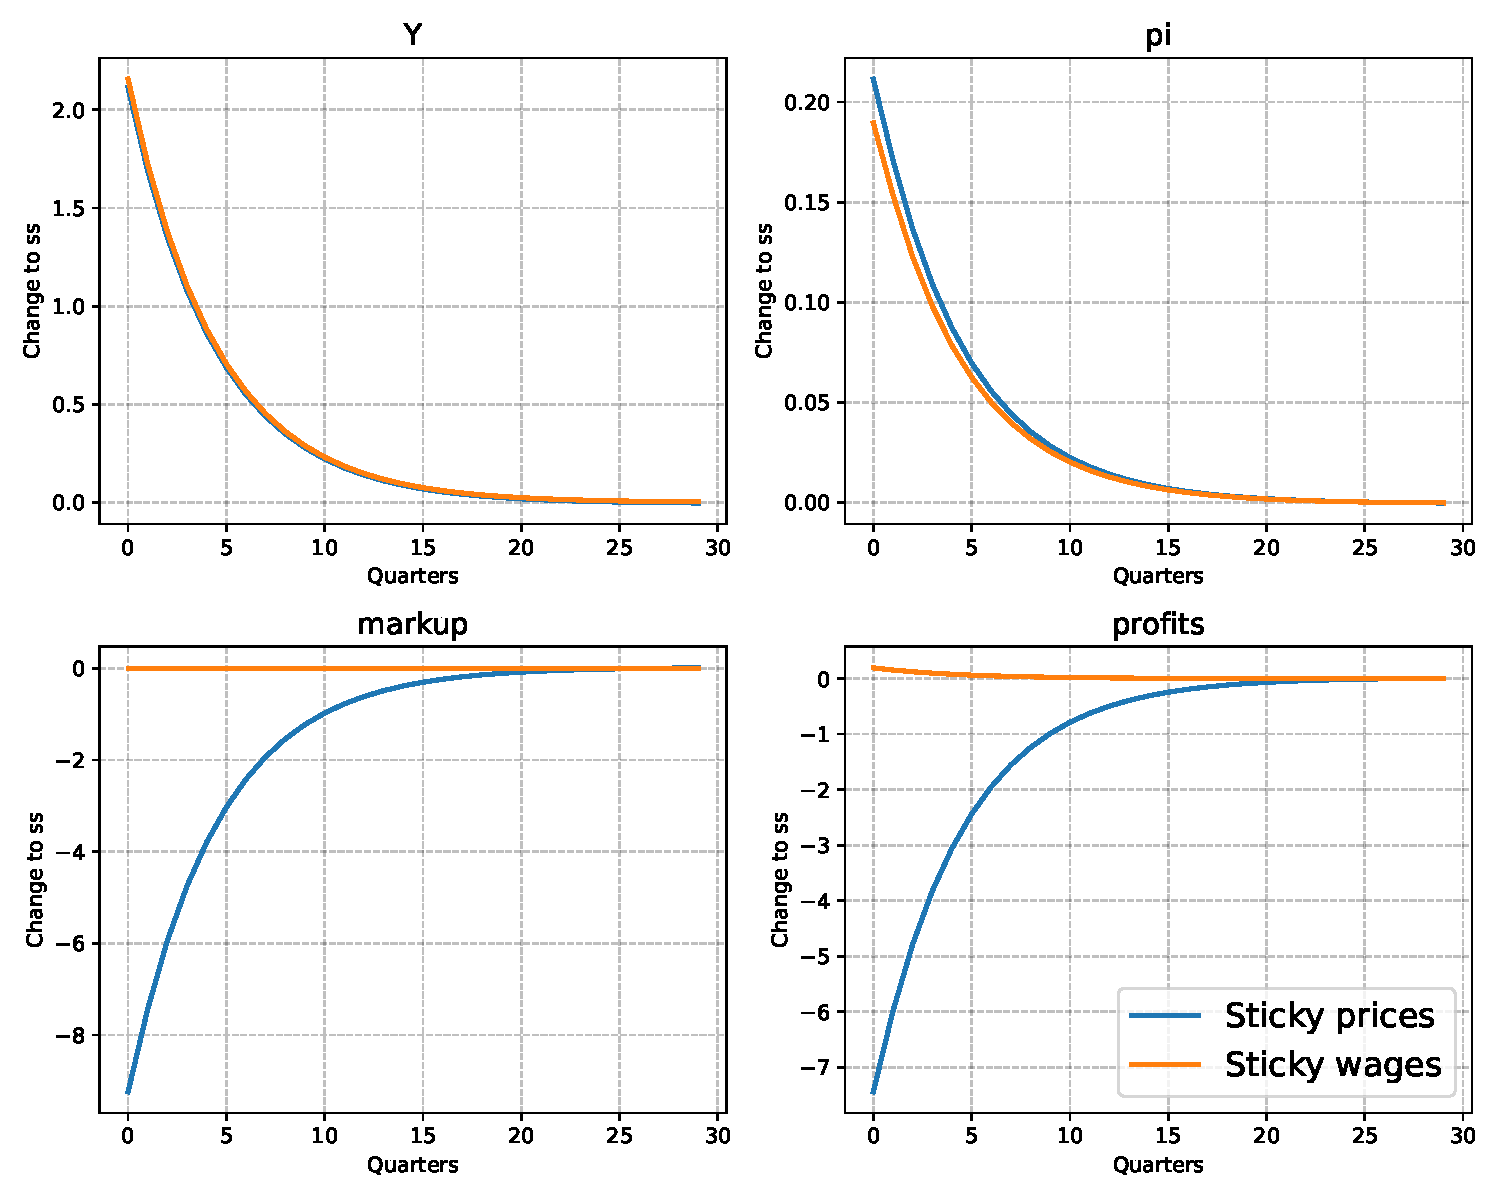
\includegraphics[width=0.5\linewidth]{figs/monpol_irf_sticky_w_p.pdf}      
\end{figure}
\end{itemize}
\end{frame}

\section{HANK}
\begin{frame}{Model elements}
\begin{itemize}
\item <+->The Heterogeneous Agent New Keynesian model
\begin{itemize}
\item Similar to standard NK model but substitute sticky prices with wages
+ HA instead of RA
\end{itemize}
\item <+->\textbf{Households}
\begin{itemize}
\item Standard HA: Face idiosynchratic income risk + borrowing constraint 
\end{itemize}
\item <+->\textbf{Firms} 
\begin{itemize}
\item Produce using labor
\end{itemize}
\item <+->\textbf{Unions}
\begin{itemize}
\item Decide on labor supply for HHs subject to wage adjustment cost
\end{itemize}
\item <+->\textbf{Mutual fund}
\begin{itemize}
\item Collect household savings and invest in available assets (today: gov'
bonds)
\end{itemize}
\item <+->\textbf{Central bank }
\item <+->\textbf{Government}
\end{itemize}
\end{frame}
%
\begin{frame}{Households}
\begin{itemize}
\item \textbf{Household problem:}
\begin{align*}
v_{t}(z_{t},a_{t-1}) & =\max_{c_{t}}\frac{c_{t}^{1-\sigma}}{1-\sigma}-\varphi\frac{\ell_{t}^{1+\nu}}{1+\nu}+\beta\mathbb{E}_{t}\left[v_{t+1}(z_{t+1},a_{t})\right]\\
\text{s.t. }a_{t}+c_{t} & =(1+r_{t}^{a})a_{t-1}+\left(1-\tau_{t}\right)w_{t}\ell_{t}z_{t}+\chi_{t}\\
\log z_{t+1} & =\rho_{z}\log z_{t}+\psi_{t+1}\,\,\,,\psi_{t}\sim\mathcal{N}(\mu_{\psi},\sigma_{\psi}),\,\mathbb{E}[z_{t}]=1\\
a_{t} & \geq0
\end{align*}
\item \textbf{Active decisions:} Consumption-saving, $c_{t}$ (and $a_{t}$)
\item \textbf{Union decision:} Labor supply, $\ell_{t}$
\item \textbf{Aggregate Consumption: $C_{t}^{hh}=\int c_{t}d\mathcal{D}_{t}$}
\item \textbf{Consumption function: $C_{t}^{hh}=C^{hh}\left(\{r_{s}^{a},\left(1-\tau_{s}\right)w_{s}\ell_{s},\chi_{s}\}_{s=0}^{\infty}\right)$}
\end{itemize}
\end{frame}
%
\begin{frame}{Firms}
\begin{itemize}
\item \textbf{Production and profits:}
\begin{align*}
Y_{t} & =\Gamma_{t}L_{t}\\
\Pi_{t} & =Y_{t}-\frac{W_{t}}{p}L_{t}
\end{align*}
\item \textbf{First order condition:}
\[
w_{t}=\Gamma_{t}
\]
\end{itemize}
\end{frame}
%
\begin{frame}{Mutual fund and assets}
\begin{itemize}
\item <+->Mutual fund collect households savings $A_{t}$ 
\item <+->Invest in available assets
\begin{itemize}
\item \textbf{Real} government bonds which pay real interest rate $r$
\end{itemize}
\item <+->\textbf{Problem}:
\[
\max_{B_{t}}\left(1+r_{t+1}\right)B_{t}-\left(1+r_{t+1}^{a}\right)A_{t}\quad\text{s.t\ensuremath{\quad B_{t}=A_{t}}}
\]
\item <+->\textbf{FOCs} (no arbitrage conditions):
\begin{align*}
1+r_{t}= & 1+r_{t}^{a}
\end{align*}
\end{itemize}
\end{frame}
%
\begin{frame}{Union}
\begin{itemize}
\item Everybody works the same:
\begin{align*}
\ell_{t} & =L_{t}^{hh}
\end{align*}
\item Maximization subject to wage adjustment cost imply a \textbf{New Keynesian
Wage (Phillips) Curve} (NKWPC or NKWC)
\[
\pi_{t}^{w}=\kappa\left(\varphi\left(L_{t}^{hh}\right)^{\nu}-\frac{1}{\mu}\left(1-\tau_{t}\right)w_{t}\left(C_{t}^{hh}\right)^{\text{-\ensuremath{\sigma}}}\right)+\beta\pi_{t+1}^{w}
\]
\end{itemize}
\end{frame}
%
\begin{frame}{Government}
\begin{itemize}
\item <+->\textbf{Spending: $G_{t}$}
\begin{align*}
B_{t} & +T_{t}+=(1+r_{t})B_{t-1}+G_{t}+\chi_{t}
\end{align*}
\item <+->where $T_{t}$ captures labor income tax revenue:
\[
T_{t}=\tau_{t}w_{t}L_{t}
\]
\item <+->In response to shocks $r_{t}$ moves which affect budget
\item <+->Need rule to ensure that government debt returns to ss in the
long run
\item <+->Potential \textbf{tax-rule:}\vspace{-1mm}
\[
\tau_{t}=\tau_{ss}+\omega\frac{B_{t-1}-B_{ss}}{Y_{ss}}
\]
\item <+->Or simply:
\[
B_{t}=B_{ss}
\]
\item <+->In which case taxes $T_{t}$ adjust fully every period to ensure
that the budget holds 
\end{itemize}
\end{frame}
%
\begin{frame}{Central bank}
\begin{itemize}
\item <+->Two options for monetary policy 
\item <+->\textbf{1. }Government bonds are nominel, CB chooses nominel
interest rate: 
\[
i_{t}=i_{ss}+\phi\pi_{t}
\]
\item <+->And fisher equation links nominal rate $i$ to real rate $r$:
\[
1+r_{t}=\frac{1+i_{t}}{1+\pi_{t+1}}
\]
\item <+->\textbf{2. Alternative:} Real rate rule. CB chooses real rate
$r_{t}$ directly 

\[
r_{t}=r_{ss}+\left(\phi-1\right)\pi_{t}
\]

\item <+->Implicit assumption: CB can control inflation. 
\begin{itemize}
\item <+->Today will study special case with >>passive<< monetary policy,
$\phi=1$ $\Rightarrow r_{t}=r_{ss}$
\end{itemize}
\item <+->Indeterminacy: Consider limit for nominal rule $i_{t}=i_{ss}+\phi\pi_{t+1}$
or assume future tightening
\end{itemize}
\end{frame}
%
\begin{frame}{Market clearing}
\begin{enumerate}
\item Asset market: $B_{t}=A_{t}^{hh}$
\item Labor market: $L_{t}=L_{t}^{hh}$
\item Goods market: $Y_{t}=C_{t}^{hh}+G_{t}$
\end{enumerate}
\end{frame}
%

\section{Fiscal Policy}
\begin{frame}{Simpler consumption function}
\begin{itemize}
\item <+->\textbf{Assumptions:}
\begin{enumerate}
\item One-period real bond
\item No lump-sum transfers, $\chi_{t}=0$
\item Fiscal policy in terms of $dG_{t}$ and $dT_{t}$ satisfying IBC (e.g.
government needs to repay excess debt $dB$ eventually)
\[
\sum_{t=0}^{\infty}(1+r_{ss})^{-t}(dG_{t}-dT_{t})=0
\]
\end{enumerate}
\item <+->\textbf{Tax-bill: $T_{t}=\tau_{t}w_{t}\int\ell_{t}z_{t}d\boldsymbol{D}_{t}=\tau_{t}\Gamma_{t}L_{t}=\tau_{t}Y_{t}$}
\item <+->\textbf{Household income:} $(1-\tau_{t})w_{t}\ell_{t}z_{t}=\underset{\equiv Z_{t}}{\underbrace{\left(Y_{t}-T_{t}\right)}}z_{t}=Z_{t}z_{t}$
\item <+->\textbf{Consumption function in sequence-space: }Simplifies to\textbf{
\[
C_{t}^{hh}=C^{hh}\left(\{Y_{s}-T_{s},r_{s}\}_{s\geq0}\right)\Rightarrow\boldsymbol{C}^{hh}=C^{hh}(\boldsymbol{Y}-\boldsymbol{T},\boldsymbol{r})=C^{hh}(\boldsymbol{Z,}\boldsymbol{r})
\]
}
\end{itemize}
\end{frame}
%
\begin{frame}{Side-note: Two-equation version in $\boldsymbol{Y}$ and $\boldsymbol{r}$}

\vspace{-5mm}\textbf{
\begin{align*}
\boldsymbol{Y} & =\boldsymbol{G}+C^{hh}(\boldsymbol{r},\boldsymbol{Y}-\boldsymbol{T})\\
\boldsymbol{r} & =\mathcal{R}\left(\boldsymbol{Y}\right)
\end{align*}
}
\begin{itemize}
\item \vspace{-7mm}\textbf{First equation:} Goods market clearing
\item \textbf{Second equation (}Firms + NKWPC\textbf{): }
\begin{enumerate}
\item Given output $\boldsymbol{Y}$, can compute $\boldsymbol{L}$
\item Firm behavior I: $\boldsymbol{\Gamma},\boldsymbol{Y}\rightarrow\boldsymbol{L},\boldsymbol{w}$
\item NKWC: $\boldsymbol{L},\boldsymbol{C},\boldsymbol{w},\boldsymbol{\tau}\rightarrow\boldsymbol{\pi^{w}}$
\item Firm behavior II: $\boldsymbol{\pi^{w}},\boldsymbol{\Gamma}\rightarrow\boldsymbol{\pi}$
\item Central bank: $\boldsymbol{\pi}\rightarrow\boldsymbol{i}$
\item Fisher: $\boldsymbol{i},\boldsymbol{\pi}\rightarrow\boldsymbol{r}$
\end{enumerate}
\item Final assumption for today: \textbf{Constant} $\boldsymbol{r}$
\begin{itemize}
\item Can replace $\boldsymbol{r}=\mathcal{R}\left(\boldsymbol{Y}\right)$
with $\boldsymbol{r}=r_{ss}$ 
\item Entire model boils down to 1 equation 
\end{itemize}
\end{itemize}
\end{frame}
%
\begin{frame}{Intertemporal Keynesian Cross}

\vspace{-5mm}
\begin{align*}
Y_{t} & =G_{t}+C_{t}^{hh}\left(\left\{ Y_{s}-T_{s}\right\} _{s=0}^{\infty}\right)\quad\quad\text{Static}\\
\boldsymbol{Y} & =\boldsymbol{G}+C^{hh}(\boldsymbol{Y}-\boldsymbol{T})\quad\quad\text{Sequence-space/vector}
\end{align*}

\begin{itemize}
\item \vspace{-2mm}\textbf{Total differentiation/linearize around ss:}
\[
dY_{t}=dG_{t}+\sum_{s=0}^{\infty}\frac{\partial C_{t}^{hh}}{\partial Z_{s}}dZ_{s}=dG_{t}+\sum_{s=0}^{\infty}\frac{\partial C_{t}^{hh}}{\partial Z_{s}}\left(dY_{s}-dT_{s}\right)
\]
\item \textbf{Intertemporal Keynesian Cross }in vector form
\begin{align*}
d\boldsymbol{Y} & =d\boldsymbol{G}+\boldsymbol{M}\left(d\boldsymbol{Y}-d\boldsymbol{T}\right)\Leftrightarrow\\
(\boldsymbol{I}-\boldsymbol{M})d\boldsymbol{Y} & =d\boldsymbol{G}-\boldsymbol{M}d\boldsymbol{T}
\end{align*}
where $M_{t,s}=\frac{\partial C_{t}^{hh}}{\partial Z_{s}}$ encodes
the entire \emph{complexity of HH behavior}
\end{itemize}
\end{frame}
%
\begin{frame}{Illustration}
\begin{itemize}
\item Writing out the IKC:
\[
\begin{aligned}\begin{bmatrix}dY_{0}\\
dY_{1}\\
dY_{2}\\
\vdots
\end{bmatrix} & =\begin{bmatrix}dG_{0}\\
dG_{1}\\
dG_{2}\\
\vdots
\end{bmatrix}+\begin{bmatrix}\frac{\partial C_{0}^{hh}}{\partial Z_{0}} & \frac{\partial C_{0}^{hh}}{\partial Z_{1}} & \frac{\partial C_{0}^{hh}}{\partial Z_{2}} & \cdots\\
\frac{\partial C_{1}^{hh}}{\partial Z_{0}} & \frac{\partial C_{1}^{hh}}{\partial Z_{1}} & \frac{\partial C_{1}^{hh}}{\partial Z_{2}} & \cdots\\
\frac{\partial C_{2}^{hh}}{\partial Z_{0}} & \frac{\partial C_{2}^{hh}}{\partial Z_{1}} & \frac{\partial C_{2}^{hh}}{\partial Z_{2}} & \cdots\\
\vdots & \vdots & \vdots & \ddots
\end{bmatrix}\left(\begin{bmatrix}dY_{0}\\
dY_{1}\\
dY_{2}\\
\vdots
\end{bmatrix}-\begin{bmatrix}dT_{0}\\
dT_{1}\\
dT_{2}\\
\vdots
\end{bmatrix}\right)\end{aligned}
\]
\end{itemize}
\end{frame}
%
\begin{frame}{iMPC matrix}
\begin{itemize}
\item <+->$\boldsymbol{M}$ is the Jacobian of aggregate $C$ w.r.t (post-tax)
labor income 
\begin{itemize}
\item Column $s$: Response of C at different dates to unit change in $Z$
at date $s$ (IRF)
\item Row $s$: Change in C at date s to change in income $Z$ at different
dates 
\[
\boldsymbol{M}=\left[\begin{array}{ccc}
\frac{\partial C_{0}^{hh}}{\partial Z_{0}} & \frac{\partial C_{0}^{hh}}{\partial Z_{1}} & \cdots\\
\frac{\partial C_{1}^{hh}}{\partial Z_{0}} & \frac{\partial C_{1}^{hh}}{\partial Z_{1}} & \cdots\\
\vdots & \vdots & \ddots
\end{array}\right]
\]
\end{itemize}
\item <+->In a quarterly model $\frac{\partial C_{0}^{hh}}{\partial Z_{0}}$
is essentially the quarterly MPC 
\begin{itemize}
\item Note: Typically define MPCs following change in lump-sum transfer
and not labor income, so not quite MPC
\end{itemize}
\end{itemize}
\end{frame}
%
\begin{frame}{iMPCs in the data}
\begin{itemize}
\item <+->What can we say about the iMPC matrix $\boldsymbol{M}$?
\begin{itemize}
\item <+-> Can say a lot about first element $\frac{\partial C_{0}^{hh}}{\partial Z_{0}}$
(see lecture 2)
\end{itemize}
\item <+-> Fagareng et al (2016) estimate dynamic response of C to income
shocks (lottery winnings)
\begin{itemize}
\item Info on first column $\left[\frac{\partial C_{0}^{hh}}{\partial Z_{0}},\frac{\partial C_{1}^{hh}}{\partial Z_{0}},\frac{\partial C_{2}^{hh}}{\partial Z_{0}},\frac{\partial C_{3}^{hh}}{\partial Z_{0}},\ldots\right]'$\\
\begin{figure}[H]     
\centering      
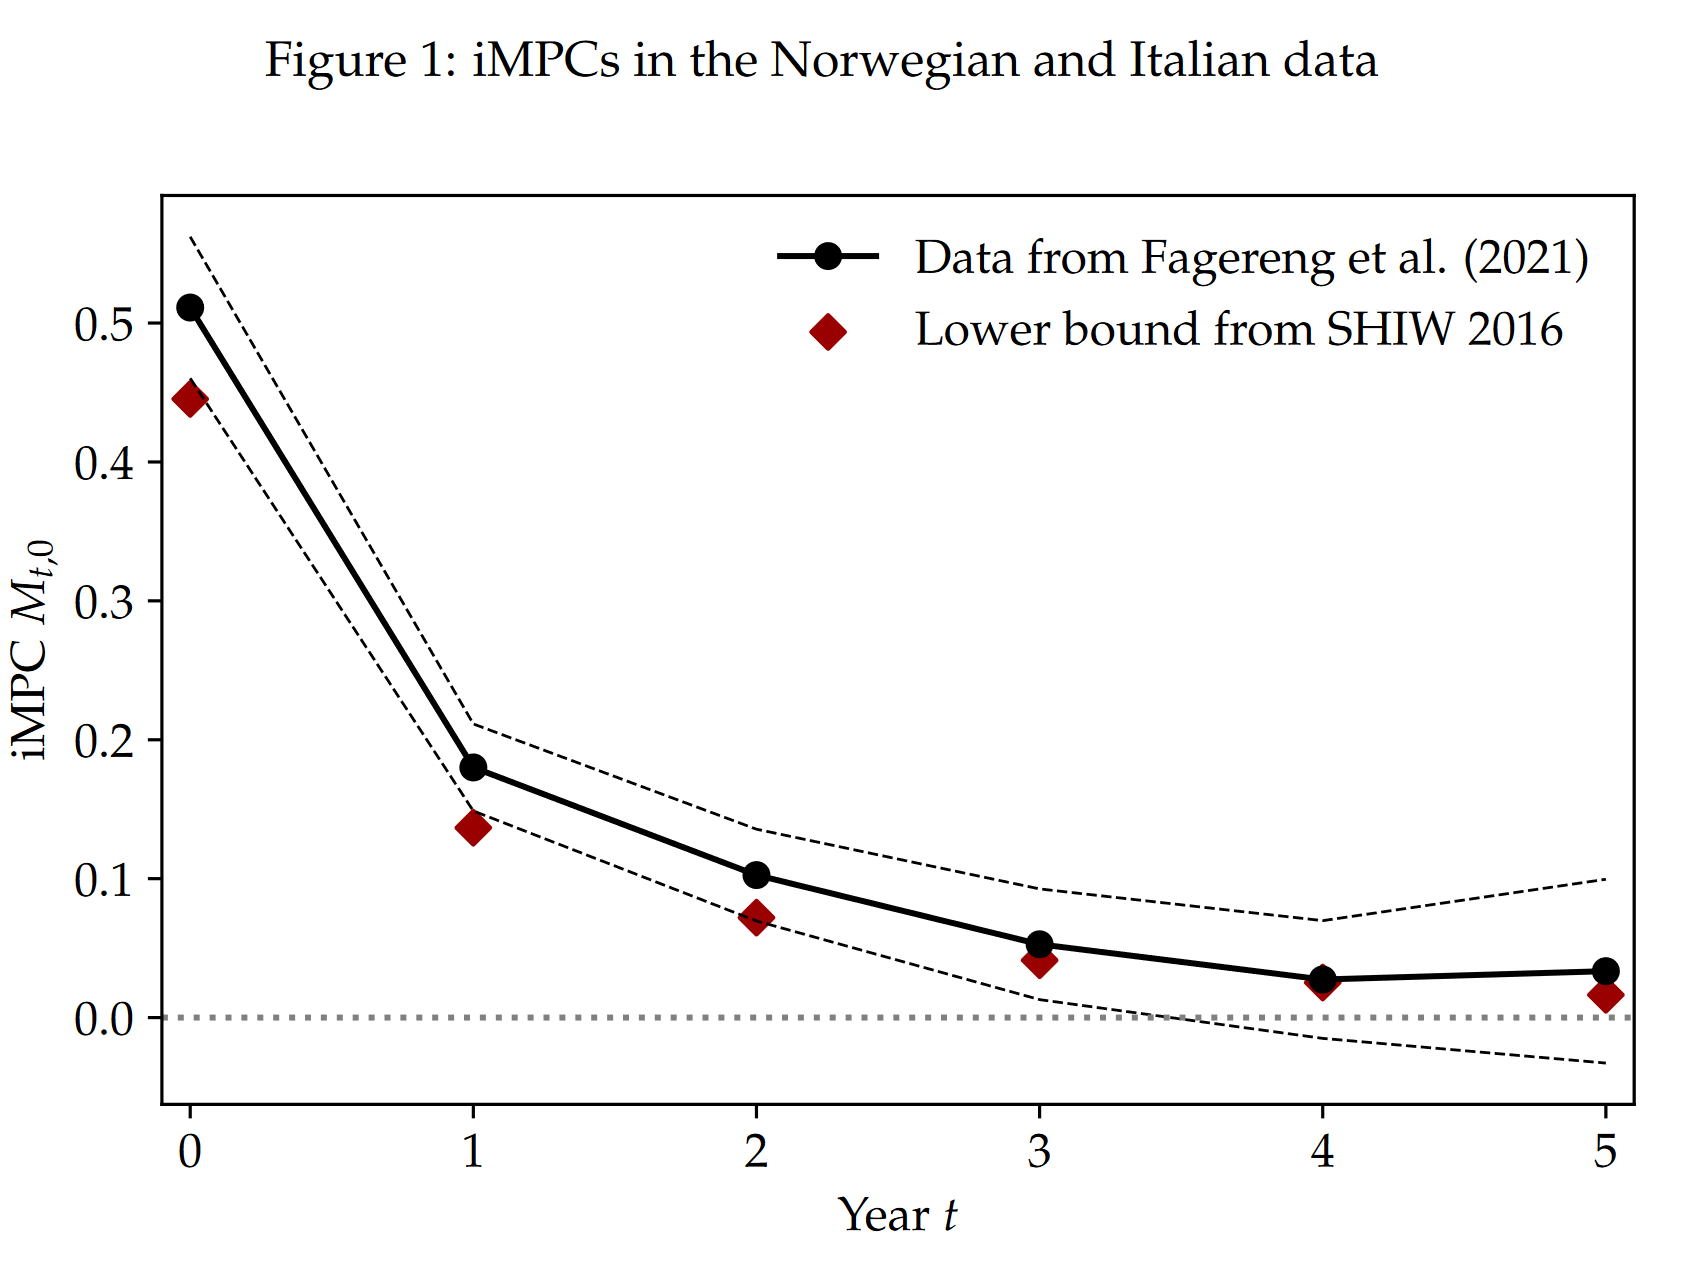
\includegraphics[width=0.5\linewidth]{figs/iMPC_data.png}      
\end{figure}
\end{itemize}
\item <+->{\footnotesize{}Very hard to say something about remaining columns
(announcement effects)}{\footnotesize\par}
\begin{itemize}
\item {\footnotesize{}Best we can do: Calibrate model to first column, get
rest of $\boldsymbol{M}$ from model}{\footnotesize\par}
\end{itemize}
\end{itemize}
\end{frame}
%
\begin{frame}{Perspective: Static Keynesian Cross}
\begin{itemize}
\item <+->\textbf{Old Keynesians:} Consumption only depends on current
income
\begin{align*}
Y_{t} & =G_{t}+C^{hh}(Y_{t}-T_{t})
\end{align*}
\item <+->\textbf{Total differentiate:}
\begin{align*}
dY_{t} & =dG_{t}+\frac{\partial C_{t}^{hh}}{\partial Z_{t}}(dY_{t}-dT_{t})\\
 & =dG_{t}+\text{mpc}\cdot(dY_{t}-dT_{t})
\end{align*}
\item <+->\textbf{Solution} 
\[
dY_{t}=dG_{t}+\frac{\text{mpc}}{1-\text{mpc}}\left(dG_{t}-dT_{t}\right)
\]
from multiplier-process $\text{mpc}\times\left(1+\text{mpc}+\text{mpc}^{2}\dots\right)=\frac{\text{mpc}}{1-\text{mpc}}$
\end{itemize}
\end{frame}
%
\begin{frame}{NPV-vector}
\begin{itemize}
\item <+->\textbf{NPV-vector: $\boldsymbol{q}\equiv[1,(1+r_{ss})^{-1},(1+r_{ss})^{-2},\dots]^{\prime}$
}- implies $\sum_{t=0}^{\infty}(1+r_{ss})^{-t}x_{t}=\boldsymbol{q}'\boldsymbol{x}$ 
\item <+->\textbf{Government: }IBC holds\textbf{\small{}
\begin{align*}
\sum_{t=0}^{\infty}(1+r_{ss})^{-t}(dG_{t}-dT_{t}) & =0\Leftrightarrow\\
\boldsymbol{q}^{\prime}(d\boldsymbol{G}-d\boldsymbol{T}) & =0
\end{align*}
}{\small\par}
\item <+->\textbf{Households: }IBC holds \textbf{\small{}
\begin{align*}
\sum_{t=0}^{\infty}(1+r_{ss})^{-t}C_{t}^{hh} & =(1+r_{ss})A_{-1}+\sum_{t=0}^{\infty}(1+r_{ss})^{-t}Z_{t}\Rightarrow\\
\sum_{t=0}^{\infty}(1+r_{ss})^{-t}M_{t,s} & =\frac{1}{(1+r)^{s}}\Rightarrow\boldsymbol{q}^{\prime}\boldsymbol{M}=\boldsymbol{q}^{\prime}\Leftrightarrow\boldsymbol{q}^{\prime}(\boldsymbol{I}-\boldsymbol{M})=\boldsymbol{0}
\end{align*}
}{\small\par}
\item <+->{\small{} Present value of $\boldsymbol{M}$ columns is 1 - HHs
must }\emph{\small{}eventually}{\small{} spend income they receive }{\small\par}
\begin{itemize}
\item $\sum_{t=0}^{\infty}\frac{MPC_{t,s}}{\left(1+r_{ss}\right)^{t-s}}=1$
\end{itemize}
\end{itemize}
\end{frame}
%
\begin{frame}{Form of unique solution}
\begin{itemize}
\item <+->\textbf{Back to IKC}: 
\[
(\boldsymbol{I}-\boldsymbol{M})d\boldsymbol{Y}=d\boldsymbol{G}-\boldsymbol{M}d\boldsymbol{T}
\]
\item <+->\textbf{Problem: }$(\boldsymbol{I}-\boldsymbol{M})^{-1}$ cannot
exist\textbf{ }because this leads to a contradiction
\begin{align*}
\boldsymbol{q}^{\prime}(\boldsymbol{I}-\boldsymbol{M})(\boldsymbol{I}-\boldsymbol{M})^{-1} & =\boldsymbol{0}(\boldsymbol{I}-\boldsymbol{M})^{-1}\Leftrightarrow\\
\boldsymbol{q}^{\prime} & =0
\end{align*}
\item <+->\textbf{Result: }If unique solution then on the form
\begin{align*}
d\boldsymbol{Y} & =\mathcal{M}(d\boldsymbol{G}-\boldsymbol{M}d\boldsymbol{T})\\
 & \,\,\,\mathcal{M}=\left(\boldsymbol{K}(\boldsymbol{I}-\boldsymbol{M})\right)^{-1}\boldsymbol{K}
\end{align*}
\item <+->\textbf{Note: }This is only an issue in infinite horizon
\begin{itemize}
\item When solving numerically we truncate at horizon T, implying that columns
in $\boldsymbol{M}$ do not exactly add to 1
\item Can then invert $(\boldsymbol{I}-\boldsymbol{M})$ (but precision
becomes worse as horizon $T$ increases)
\end{itemize}
\end{itemize}
\end{frame}
%
\begin{frame}{Response of consumption}

\begin{align*}
d\boldsymbol{Y} & =d\boldsymbol{G}+\boldsymbol{M}(d\boldsymbol{Y}-d\boldsymbol{T})\Leftrightarrow\\
d\boldsymbol{Y}-d\boldsymbol{G} & =\boldsymbol{M}(d\boldsymbol{G}-d\boldsymbol{T})+\boldsymbol{M}(d\boldsymbol{Y}-d\boldsymbol{G})\Leftrightarrow\\
(I-\boldsymbol{M})\left(d\boldsymbol{Y}-d\boldsymbol{G}\right) & =\boldsymbol{M}(d\boldsymbol{G}-d\boldsymbol{T})\Leftrightarrow\\
d\boldsymbol{Y}-d\boldsymbol{G} & =\mathcal{M}\boldsymbol{M}(d\boldsymbol{G}-d\boldsymbol{T})\Leftrightarrow\\
d\boldsymbol{C} & =\mathcal{M}\boldsymbol{M}(d\boldsymbol{G}-d\boldsymbol{T})
\end{align*}

\end{frame}
%
\begin{frame}{Fiscal multipliers}

\vspace{-2mm}
\[
d\boldsymbol{Y}=d\boldsymbol{G}+\underset{d\boldsymbol{C}}{\underbrace{\mathcal{M}\boldsymbol{M}(d\boldsymbol{G}-d\boldsymbol{T})}}
\]
\begin{itemize}
\item \vspace{-5mm}\textbf{Balanced budget multiplier: }
\[
d\boldsymbol{G}=d\boldsymbol{T}\Rightarrow d\boldsymbol{Y}=d\boldsymbol{G},d\boldsymbol{C}=0
\]

Note: Central that income and taxes affect household income proportionally
in exactly the same way $=$ no redistribution
\item \vspace{2mm}\textbf{Deficit multiplier:} $d\boldsymbol{G}\neq d\boldsymbol{T}$
\begin{enumerate}
\item Potentially fiscal multiplier \textbf{above} 1
\item Larger effect of $d\boldsymbol{G}$ than $d\boldsymbol{T}$
\item \emph{Numerical results needed}
\end{enumerate}
\end{itemize}
\end{frame}
%
\begin{frame}{Fiscal multiplier}

\textbf{Impact-multiplier:} 
\[
\frac{\partial Y_{0}}{\partial G_{0}}
\]
\textbf{Cumulative-multiplier: }
\[
\frac{\sum_{t=0}^{\infty}(1+r_{ss})^{-t}dY_{t}}{\sum_{t=0}^{\infty}(1+r_{ss})^{-t}dG_{t}}
\]

\end{frame}
%
\begin{frame}{Comparison with RA model}
\begin{itemize}
\item \textbf{From lecture 1:} $\beta(1+r_{ss})=1$ implies
\[
C_{t}=(1-\beta)\sum_{s=0}^{\infty}\beta^{s}Y_{t+s}^{hh}+r_{ss}a_{-1}
\]
\item The \textbf{iMPC-matrix} becomes ($\boldsymbol{1}$ is a square matrix
of 1's)
\[
\boldsymbol{M}^{RA}=\left[\begin{array}{cccc}
(1-\beta) & (1-\beta)\beta & (1-\beta)\beta^{2} & \cdots\\
(1-\beta) & (1-\beta)\beta & (1-\beta)\beta^{2} & \cdots\\
(1-\beta) & (1-\beta)\beta & (1-\beta)\beta^{2} & \cdots\\
\vdots & \vdots & \vdots & \ddots
\end{array}\right]=(1-\beta)\boldsymbol{1}\boldsymbol{q}^{\prime}
\]
\item \textbf{Consumption response} is zero 
\begin{align*}
d\boldsymbol{C}^{\boldsymbol{RA}} & =\mathcal{M}\boldsymbol{M}^{\boldsymbol{RA}}(d\boldsymbol{G}-d\boldsymbol{T})\\
 & =\mathcal{M}(1-\beta)\boldsymbol{1}\boldsymbol{q}^{\prime}(d\boldsymbol{G}-d\boldsymbol{T})\\
 & =\boldsymbol{0}\Leftrightarrow d\boldsymbol{Y}=d\boldsymbol{G}
\end{align*}
\item \textbf{Fiscal multiplier is 1}
\begin{itemize}
\item Note: Lower when real rate responds
\end{itemize}
\end{itemize}
\end{frame}
%
\begin{frame}{Details on matrix formulation}

{\footnotesize{}
\begin{align*}
(1-\beta)\boldsymbol{1}\boldsymbol{q}^{\prime} & =\left[\begin{array}{cccc}
(1-\beta) & (1-\beta) & (1-\beta) & \cdots\\
(1-\beta) & (1-\beta) & (1-\beta) & \cdots\\
(1-\beta) & (1-\beta) & (1-\beta) & \cdots\\
\vdots & \vdots & \vdots & \ddots
\end{array}\right]\left[\begin{array}{cccc}
1 & (1+r_{ss})^{-1} & (1+r_{ss})^{-2} & \cdots\end{array}\right]\\
 & =\left[\begin{array}{cccc}
(1-\beta) & (1-\beta) & (1-\beta) & \cdots\\
(1-\beta) & (1-\beta) & (1-\beta) & \cdots\\
(1-\beta) & (1-\beta) & (1-\beta) & \cdots\\
\vdots & \vdots & \vdots & \ddots
\end{array}\right]\left[\begin{array}{cccc}
1 & \beta & \beta^{2} & \cdots\end{array}\right]\\
 & =\left[\begin{array}{cccc}
(1-\beta) & (1-\beta)\beta & (1-\beta)\beta^{2} & \cdots\\
(1-\beta) & (1-\beta)\beta & (1-\beta)\beta^{2} & \cdots\\
(1-\beta) & (1-\beta)\beta & (1-\beta)\beta^{2} & \cdots\\
\vdots & \vdots & \vdots & \ddots
\end{array}\right]
\end{align*}
}{\footnotesize\par}
\end{frame}
%
\begin{frame}{TANK}
\begin{itemize}
\item <+->\textbf{RANK} cannot produce fiscal multipliers above 1 because
it features ricardian equivalence
\item <+->Large litterature on Two Agent New Keyniesan models (TANK) starting
with Campbell and Mankiw (1989)
\begin{itemize}
\item Share $1-\lambda$ is unconstrained; Always on Euler (Ricardian, permanent
income HHs, optimizing HHs)
\item Share $\lambda$ is constrained (no savings) and consume entire income
each period, $MPC=1$ (hand to mouth)
\end{itemize}
\item <+-> $\boldsymbol{M}$ matrix is:
\[
\boldsymbol{M}^{TA}=\left(1-\lambda\right)\boldsymbol{M}^{RA}+\lambda\boldsymbol{I}
\]
\item <+->Simple to implement+tractable, but some drawbacks
\begin{itemize}
\item No intertemporal MPCs
\item Extremely stylized level of inequality 
\item Hard to connect to micro data 
\item No precautionary saving
\end{itemize}
\end{itemize}
\end{frame}
%
\begin{frame}{Comparison with TANK model}
\begin{itemize}
\item <+->\textbf{Hand-to-Mouth (HtM) households:} $\lambda$ share have
$C_{t}=Y_{t}^{hh}$
\[
\boldsymbol{M}^{TA}=(1-\lambda)\boldsymbol{M}^{RA}+\lambda\boldsymbol{I}
\]
\item <+->\textbf{Intertemporal Keynesian Cross} becomes
\begin{align*}
d\boldsymbol{Y} & =d\boldsymbol{G}+\boldsymbol{M}^{TA}\left(d\boldsymbol{Y}-d\boldsymbol{T}\right)\\
(\boldsymbol{I}-\boldsymbol{M}^{TA})d\boldsymbol{Y} & =d\boldsymbol{G}-\boldsymbol{M}^{TA}d\boldsymbol{T}\\
(\boldsymbol{I}-\boldsymbol{M}^{RA})d\boldsymbol{Y} & =\frac{1}{1-\lambda}\left[d\boldsymbol{G}-\lambda d\boldsymbol{T}\right]-\boldsymbol{M}^{RA}d\boldsymbol{T}
\end{align*}
\item <+->\textbf{Solution:}
\[
d\boldsymbol{Y}=d\boldsymbol{G}+\frac{\lambda}{1-\lambda}\left[d\boldsymbol{G}-d\boldsymbol{T}\right]
\]
\item <+->\textbf{Amplification} of fiscal policy with deficit financing
$d\boldsymbol{G}>d\boldsymbol{T}$
\begin{itemize}
\item Size of amplification increasing in share of constrained agents $\lambda$
\item Solution \textbf{very }similar to static, old Keynesian cross (multiplier:
$\frac{\text{mpc}}{1-\text{mpc}}$)
\end{itemize}
\end{itemize}
\end{frame}
%
\begin{frame}{TANK Proof}
\begin{itemize}
\item {\footnotesize{}In TANK we have:
\begin{align*}
d\boldsymbol{Y} & =d\boldsymbol{G}+\boldsymbol{M}^{TA}\left(d\boldsymbol{Y}-d\boldsymbol{T}\right)\\
(\boldsymbol{I}-\boldsymbol{M}^{TA})d\boldsymbol{Y} & =d\boldsymbol{G}-\boldsymbol{M}^{TA}d\boldsymbol{T}\\
(\boldsymbol{I}-\boldsymbol{M}^{RA})d\boldsymbol{Y} & =\frac{1}{1-\lambda}\left[d\boldsymbol{G}-\lambda d\boldsymbol{T}\right]-\boldsymbol{M}^{RA}d\boldsymbol{T}\\
d\boldsymbol{Y} & =\boldsymbol{M}^{RA}d\boldsymbol{Y}-\boldsymbol{M}^{RA}d\boldsymbol{T}+\frac{1}{1-\lambda}\left[d\boldsymbol{G}-\lambda d\boldsymbol{T}\right]\\
d\boldsymbol{Y} & =d\tilde{\boldsymbol{G}}+\boldsymbol{M}^{RA}\left(d\boldsymbol{Y}-d\boldsymbol{T}\right)
\end{align*}
}{\footnotesize\par}
\item {\footnotesize{}where $d\tilde{\boldsymbol{G}}=\frac{1}{1-\lambda}\left[d\boldsymbol{G}-\lambda d\boldsymbol{T}\right]$}{\footnotesize\par}
\item {\footnotesize{}Recall that in RANK $d\boldsymbol{Y}=d\boldsymbol{G}+\boldsymbol{M}^{RA}(d\boldsymbol{Y}-d\boldsymbol{T})$
with solution $d\boldsymbol{Y}=d\boldsymbol{G}$ thus implying $d\boldsymbol{Y}=d\tilde{\boldsymbol{G}}$
in TANK:
\begin{align*}
d\boldsymbol{Y} & =\frac{1}{1-\lambda}\left[d\boldsymbol{G}-\lambda d\boldsymbol{T}\right]\\
d\boldsymbol{Y} & =d\boldsymbol{G}-d\boldsymbol{G}+\frac{1}{1-\lambda}\left[d\boldsymbol{G}-\lambda d\boldsymbol{T}\right]\\
d\boldsymbol{Y} & =d\boldsymbol{G}+\frac{\lambda}{1-\lambda}\left[d\boldsymbol{G}-\lambda d\boldsymbol{T}\right]
\end{align*}
}{\footnotesize\par}
\end{itemize}
\end{frame}
%
\begin{frame}{Cumulative multiplier still one}
\begin{align*}
\frac{\boldsymbol{q}^{\prime}d\boldsymbol{Y}}{\boldsymbol{q}^{\prime}d\boldsymbol{G}} & =\frac{\boldsymbol{q}^{\prime}d\boldsymbol{G}_{t}+\frac{\lambda}{1-\lambda}\boldsymbol{q}^{\prime}\left[d\boldsymbol{G}-d\boldsymbol{T}\right]}{\boldsymbol{q}^{\prime}d\boldsymbol{G}}\\
 & =1
\end{align*}
\end{frame}
%
\begin{frame}{Jacobian columns}
\begin{itemize}
\item TANK produces positive C response, fiscal multiplier above 1 - do
we need HANK?
\item Plot columns of $\boldsymbol{M}$ in TANK, HANK + other models
\begin{itemize}
\item Recall columns: dynamic \textbf{$C$} response to change in $Z$ at
various dates\\
\begin{figure}[H]     
\centering      
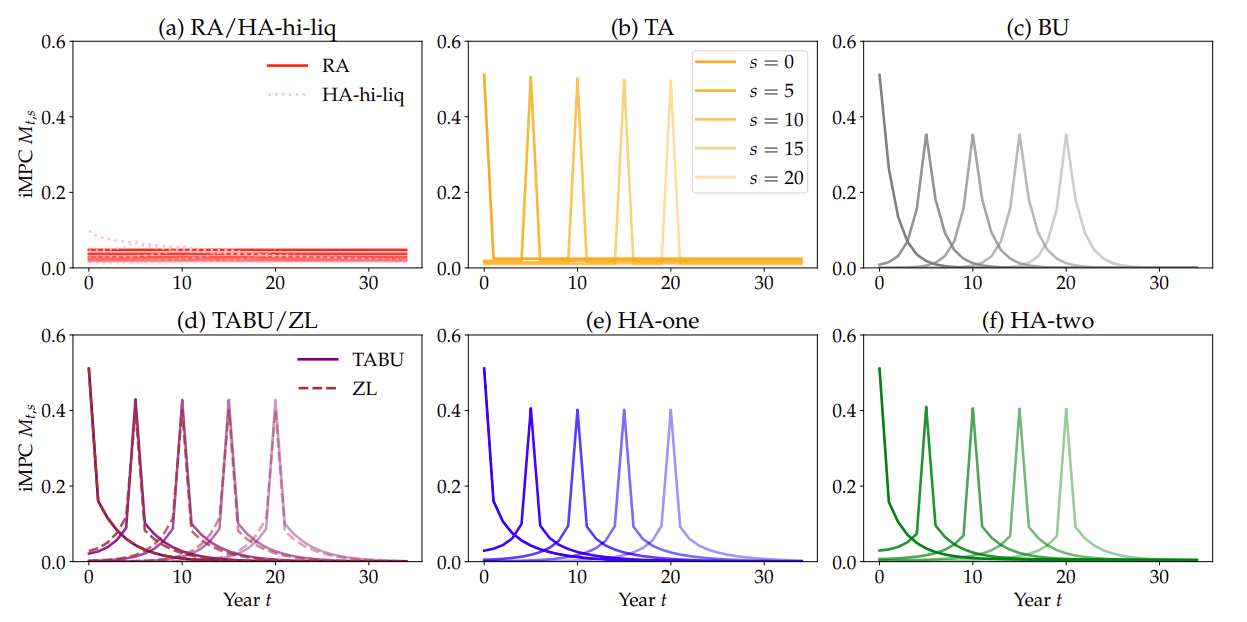
\includegraphics[width=0.9\linewidth]{figs/IKCMColumnsFull.png}      
\end{figure}
\end{itemize}
\end{itemize}
\end{frame}
%
\begin{frame}{iMPCs in models}

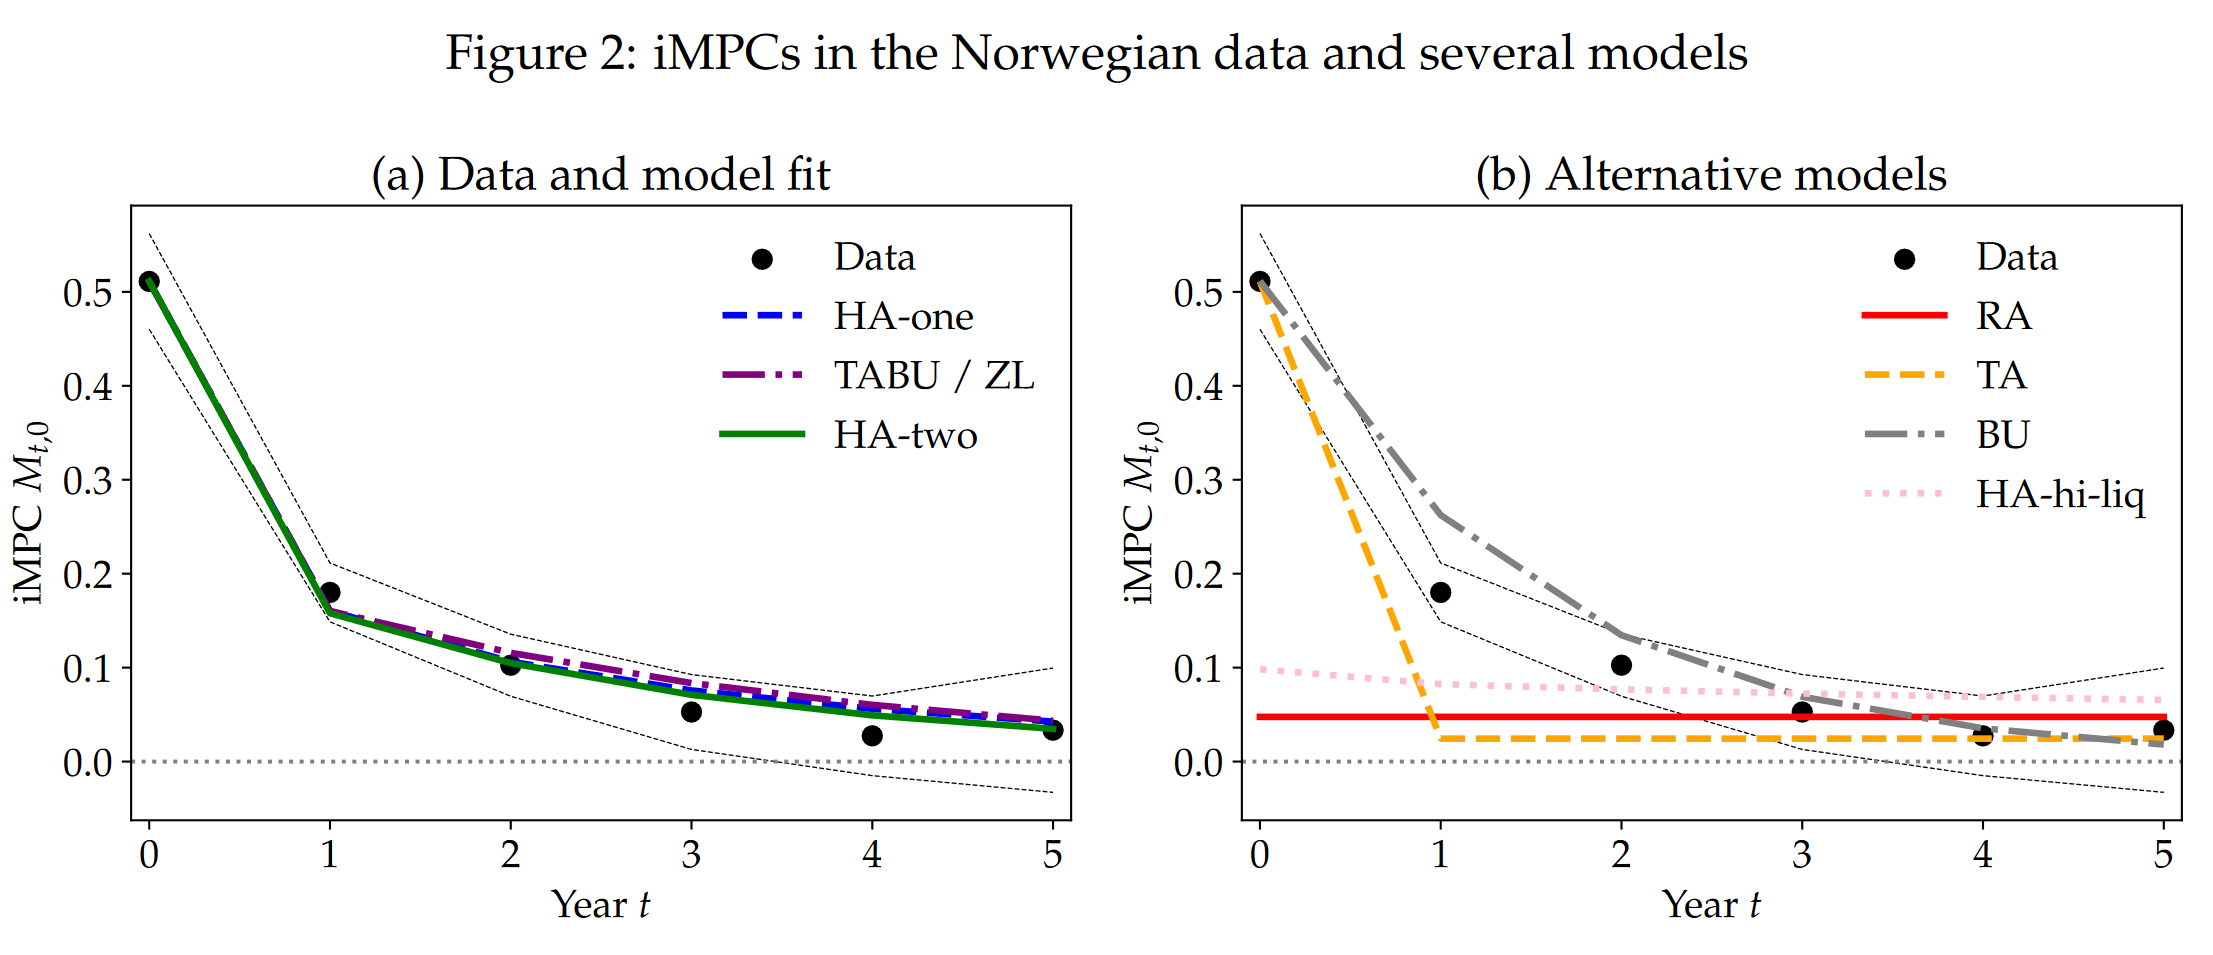
\includegraphics[width=1\textwidth]{figs/iMPC_models}
\end{frame}
%
\begin{frame}{Multipliers and debt-financing}

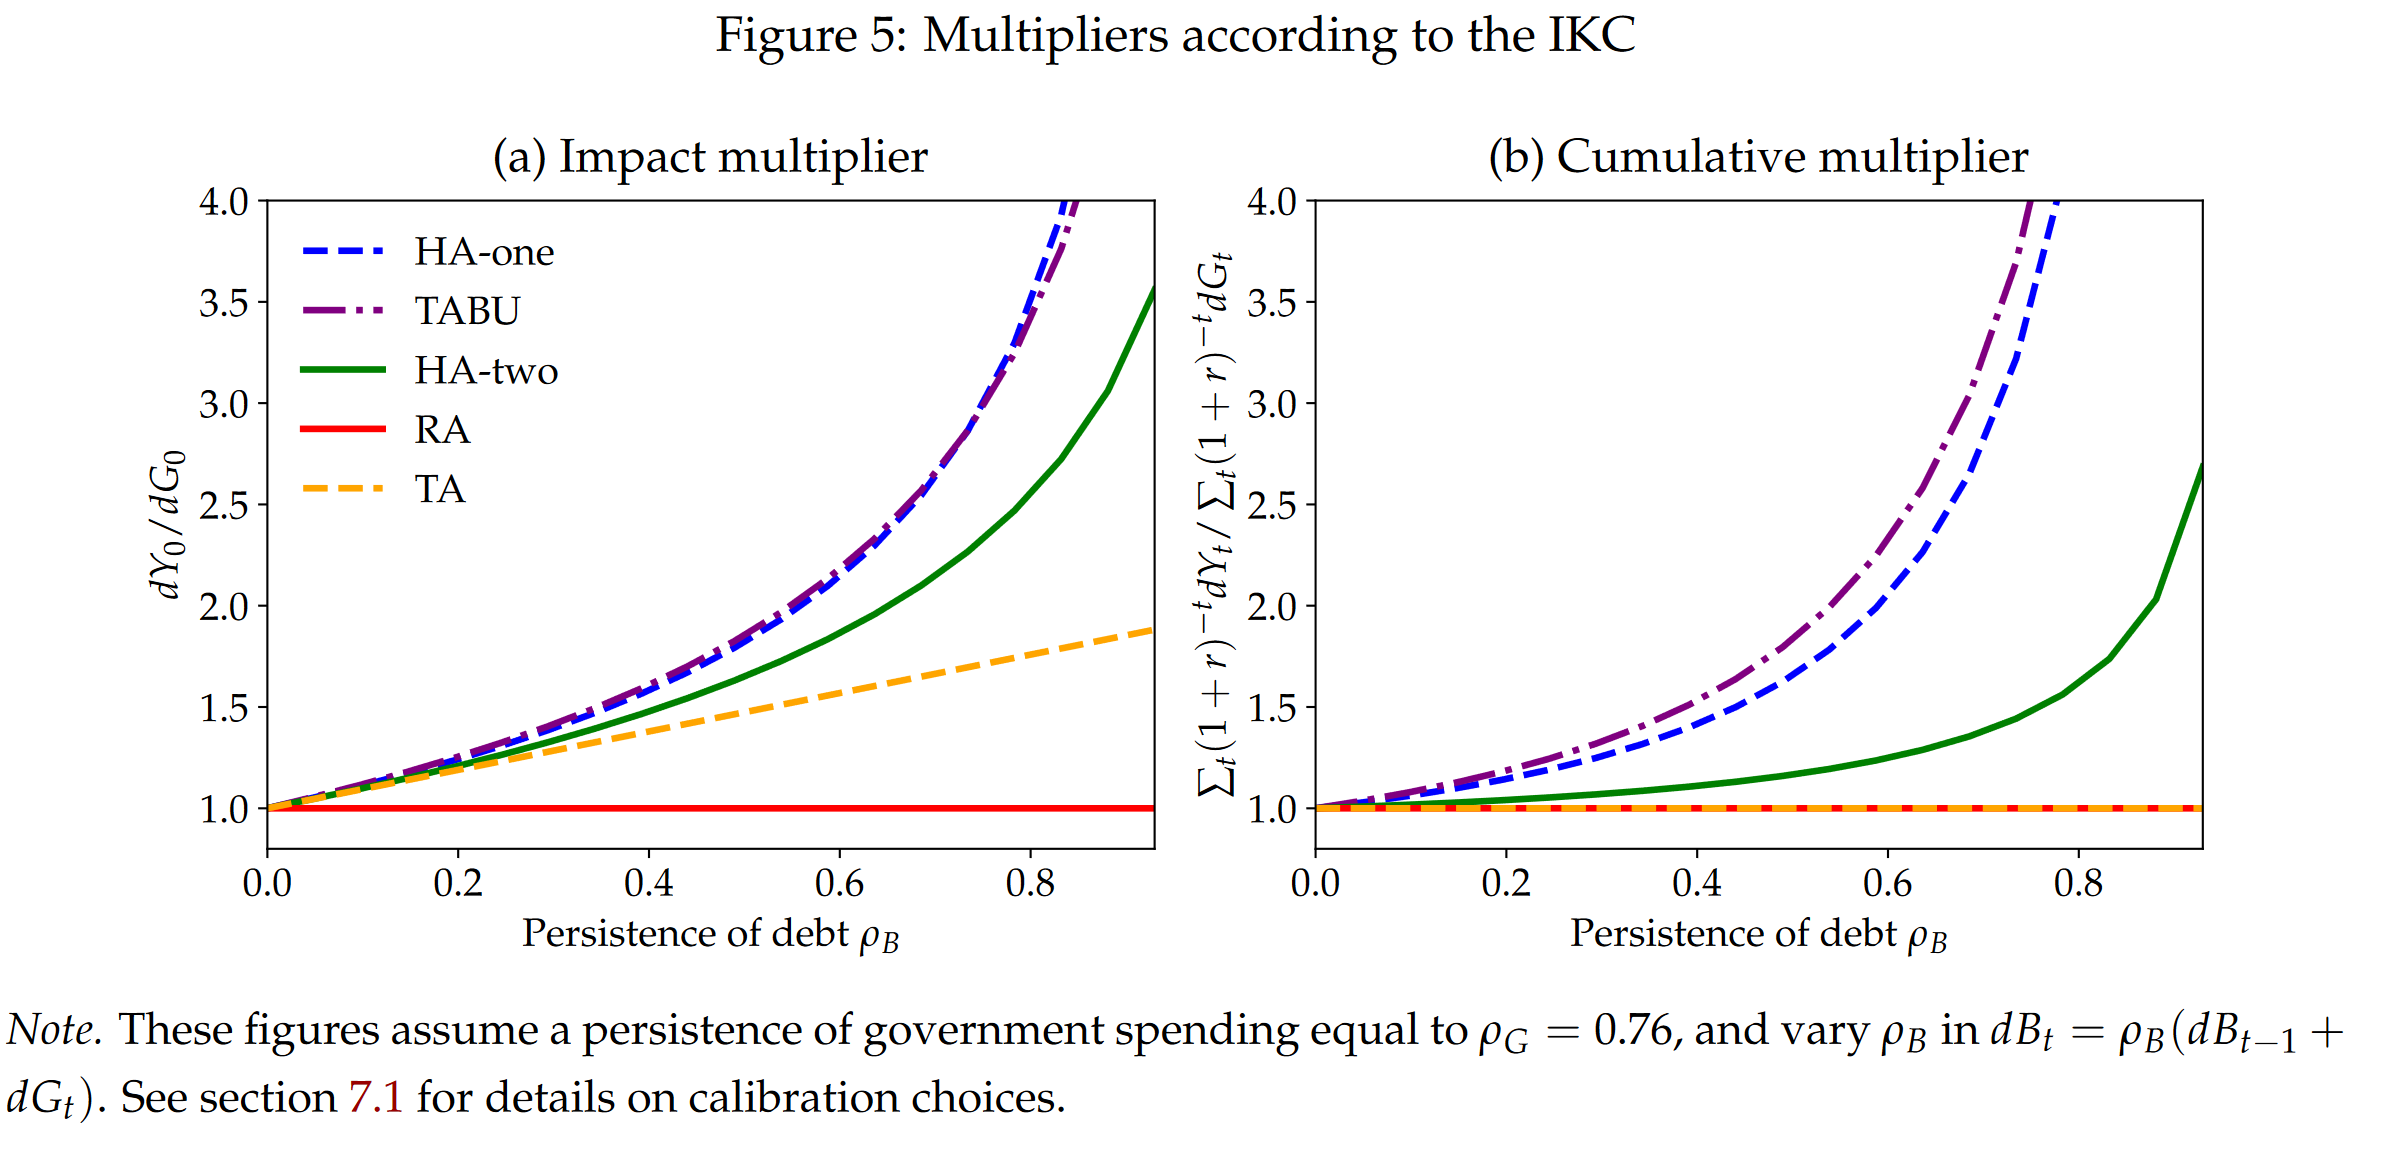
\includegraphics[width=1\textwidth]{figs/multiplier}
\end{frame}
%
\begin{frame}{Summary in table}
\begin{itemize}
\item Summary:\\
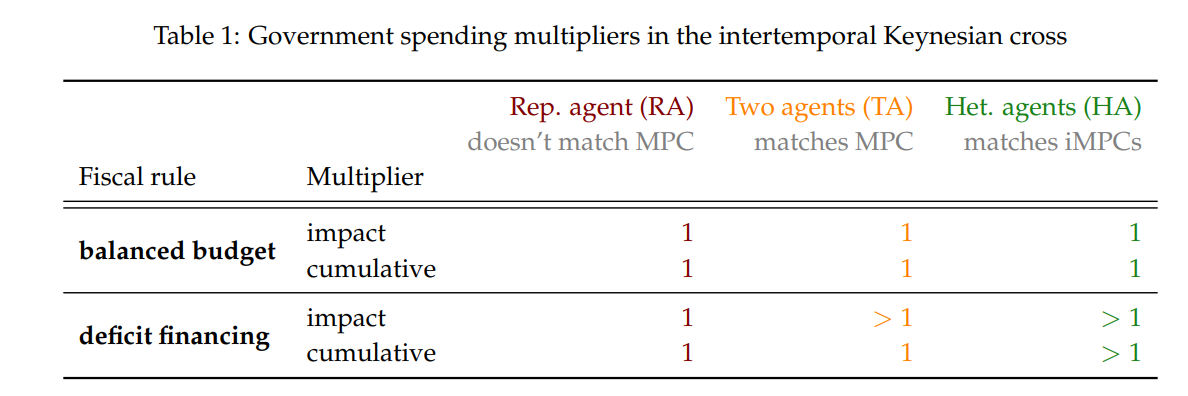
\includegraphics[width=1\textwidth]{figs/IKCTable1}
\end{itemize}
\end{frame}
%
\begin{frame}{Interest rate effects}
\begin{itemize}
\item <+->We assumed real bonds for tractablity - In reality, bonds are
typically \textbf{nominal:}
\item \textbf{
\begin{align*}
\left(1+r_{t}\right)B_{t-1}\quad & \text{versus}\quad\frac{1+i_{t-1}}{1+\pi_{t}}B_{t-1}
\end{align*}
}
\item <+->\textbf{Fisher}: $\left(1+r_{t}\right)=\frac{1+i_{t-1}}{1+\pi_{t}}\approx r_{t}=i_{t-1}-\pi_{t}$
\item <+->Even if CB keeps ex-ante real rate constant $i_{t}=i_{ss}+\pi_{t+1}$
real returns on bonds will differ in period 0:
\item <+->Period 0:
\[
\frac{1+i_{ss}}{1+\pi_{0}}B_{ss}
\]
\item <+->Period 1:
\[
\frac{1+i_{0}}{1+\pi_{1}}B_{0}=\left(1+r\right)B_{0}
\]
\item <+->With nominal bonds \textbf{surprise inflation} affects returns
- implies capital for households in period 0 
\begin{itemize}
\item Positive fiscal shock generates inflation, so \textbf{negative} effect
on return
\end{itemize}
\end{itemize}
\end{frame}
%
\begin{frame}{Generalized IKC}
\begin{itemize}
\item \textbf{Budget constraint} can be written with initial capital gain
\[
a_{t}+c_{t}=(Y_{t}-T_{t})z_{t}+\chi_{t}+\begin{cases}
(1+r_{t-1}^{a})a_{t-1} & \text{if }t>0\\
(1+r_{ss}+\text{cap}_{0})a_{t-1} & \text{if }t=0
\end{cases}
\]

\begin{enumerate}
\item Real bond: $\text{cap}_{0}=0$
\item Nominal bond: 
\[
\text{cap}_{0}=\frac{(1+r_{ss})(1+\pi_{ss})}{1+\pi_{0}}-(1+r_{ss})
\]
\end{enumerate}
\end{itemize}
\end{frame}
%
\begin{frame}{Generalized IKC}
\begin{itemize}
\item \textbf{Consumption-function $\boldsymbol{C}^{hh}=C^{hh}(\boldsymbol{r},\boldsymbol{Y}-\boldsymbol{T},\text{cap}_{0})$
}implies
\begin{align*}
d\boldsymbol{C}^{hh} & =\boldsymbol{M}^{r}d\boldsymbol{r}+\boldsymbol{M}(d\boldsymbol{Y}-d\boldsymbol{T})+\boldsymbol{m}^{\text{cap}}\text{cap}_{0}
\end{align*}
where
\[
\boldsymbol{M}_{t,s}^{r}=\left[\frac{\partial C_{t}^{hh}}{\partial r_{s}}\right],\boldsymbol{m}_{t}^{\text{cap}}=\left[\frac{\partial C_{t}^{hh}}{\partial\text{cap}_{0}}\right]
\]
\item Capital return effect is negative - can this overturn fiscal multiplier
> 1?
\begin{itemize}
\item No - entries in $\boldsymbol{M}$ are large
\item Entries in $\boldsymbol{m}^{\text{cap}}$ are \textbf{small}
\end{itemize}
\item MPC out of capital gains approximatly 1-4\% per year
\end{itemize}
\end{frame}
%
\begin{frame}{Fiscal policy in HANK - litterature}
\begin{itemize}
\item Seminal paper:\textbf{ Intertemporal Keynesian Cross}
\item \textbf{Many} other interesting papers:
\item McKay and Reis - \emph{The role of automatic stabilizers in the US
business cycle} (2016)
\begin{itemize}
\item Analyze the role of automatic stabilizers in a HANK model 
\end{itemize}
\item Bayer, Born, Luetticke - \emph{The liquidity channel of fiscal policy}
(2023)
\begin{itemize}
\item Role of liquid and illiquid effects of fiscal policy
\end{itemize}
\item Hagedorn, Manovskii, and Mitman - \emph{The fiscal multiplier} (2019)
\begin{itemize}
\item Systematic evaluation of multiplier in HANK + ZLB 
\end{itemize}
\item Druedahl, Ravn, Sunder-Plassmann, Sundram, \& Waldstrøm - \emph{Fiscal
Multipliers in Small Open Economies With Heterogeneous Households
(2024)}
\begin{itemize}
\item Generalize to small open economies 
\end{itemize}
\end{itemize}
\end{frame}
%

\section{Exercise}
\begin{frame}{Exercise}

{\small{}Consider the standard HANK model outlined in section 2}{\small\par}
\begin{enumerate}
\item {\small{}Compute and plot selected columns of the household Jacobian
of $C$ w.r.t $Z,r,\chi$ }\\
{\small{}Hint: use $\text{model.\_compute\_jac\_hh()}$to compute
the jacobians. You can find the results in $\text{model.jac\_hh}$}{\small\par}
\begin{enumerate}
\item {\small{}Are the MPCs out of labor income $Z$ and a transfer $\chi$
different? why?}{\small\par}
\end{enumerate}
\item {\small{}Compute IRFs to a deficit financed $(\omega=0.1$) and tax
financed $(\omega$ large) fiscal spending shock. Compare the responses.}{\small\par}
\item {\small{}Compute the output IRF $d\boldsymbol{Y}$ using the fomula
$d\boldsymbol{Y}=d\boldsymbol{G}+\mathcal{M}\boldsymbol{M}\left[d\boldsymbol{G}-d\boldsymbol{T}\right]$
where $\mathcal{M}=\left(\boldsymbol{I}-\boldsymbol{M}\right)^{-1}$.
Check that you get the same as when using $\text{model.find\_IRFs()}$}{\small\par}
\item {\small{}Redo Q2 with active monetary policy, $\phi_{\pi}=1.5$. How
does the fiscal multiplier change? }{\small\par}
\item {\small{}Redo Q2 with active monetary policy }\emph{\small{}and }{\small{}a
flatter NKWPC, $\kappa=0.01$. How does the fiscal multiplier change? }{\small\par}
\end{enumerate}
\end{frame}
%

\section{Summary}
\begin{frame}{Summary and next week}
\begin{itemize}
\item \textbf{Today: }Fiscal policy in a HANK model with sticky wages
\item \textbf{Next week: }Assignment workshop
\item \textbf{Homework:}
\begin{enumerate}
\item Work on exercise
\item Work on assignment 
\end{enumerate}
\end{itemize}
\end{frame}
%

\end{document}
